\documentclass[a4paper,12pt]{article}
\usepackage[utf8]{vietnam}
\usepackage{hyperref}
\usepackage{graphicx}
\usepackage{xcolor}
\usepackage{subfigure}
\usepackage{float}
\usepackage{caption}
\usepackage{placeins}
\makeatletter
\setlength{\@fptop}{0pt}
\makeatother
\hypersetup{
	pdfborder = {0 0 0}
}
\title{\textbf{Báo cáo tuần 11 \\ Thực hành kiến trúc máy tính}}
\author{Họ tên: Phan Minh Anh Tuấn \\ MSSV: 20205227}
\date{}
\begin{document}
	\maketitle
	\tableofcontents
	\newpage
\section{Assignment 1}
	\subsection{Phân tích đề bài}
	Nhận dạng phím được bấm và in mã của số đó trên console. \\
	\textbf{MSSV:} 20205227 => Kiểm tra hàng 1 và hàng 2.
	\subsection{Triển khai MIPS}
	\FloatBarrier
	\begin{figure}[ht!]
		\centerline{\fbox{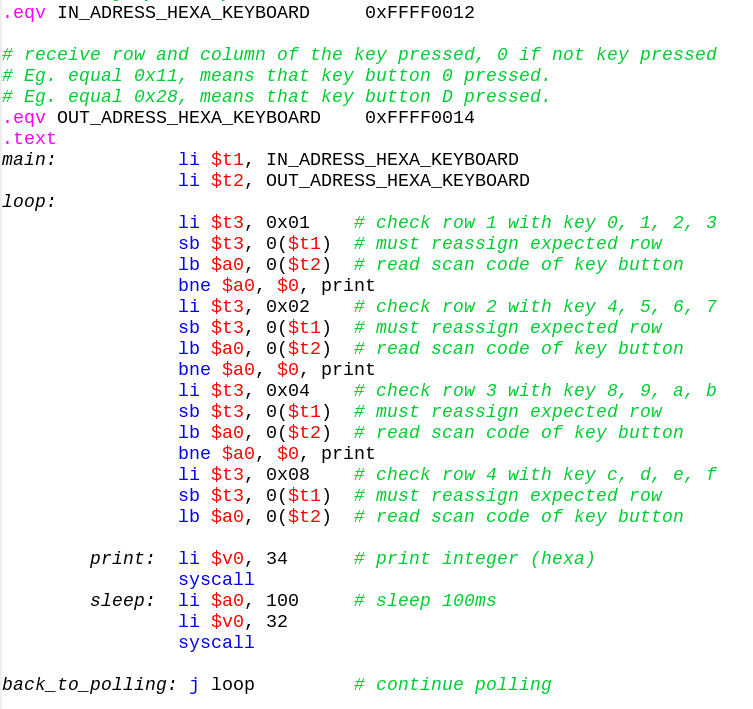
\includegraphics[width=1\textwidth]{ass1/code.png}}}
		\caption{Code của Assignment 1}
		\label{fig:ass1}
	\end{figure}
	\noindent
	Đoạn mã thực hiện theo cơ chế POOLING: Vòng lặp vô hạn để đọc kí tự được nhấn.
	\clearpage
	\subsection{Kết quả}
	\FloatBarrier
	\begin{figure}[ht!]
		\centerline{\fbox{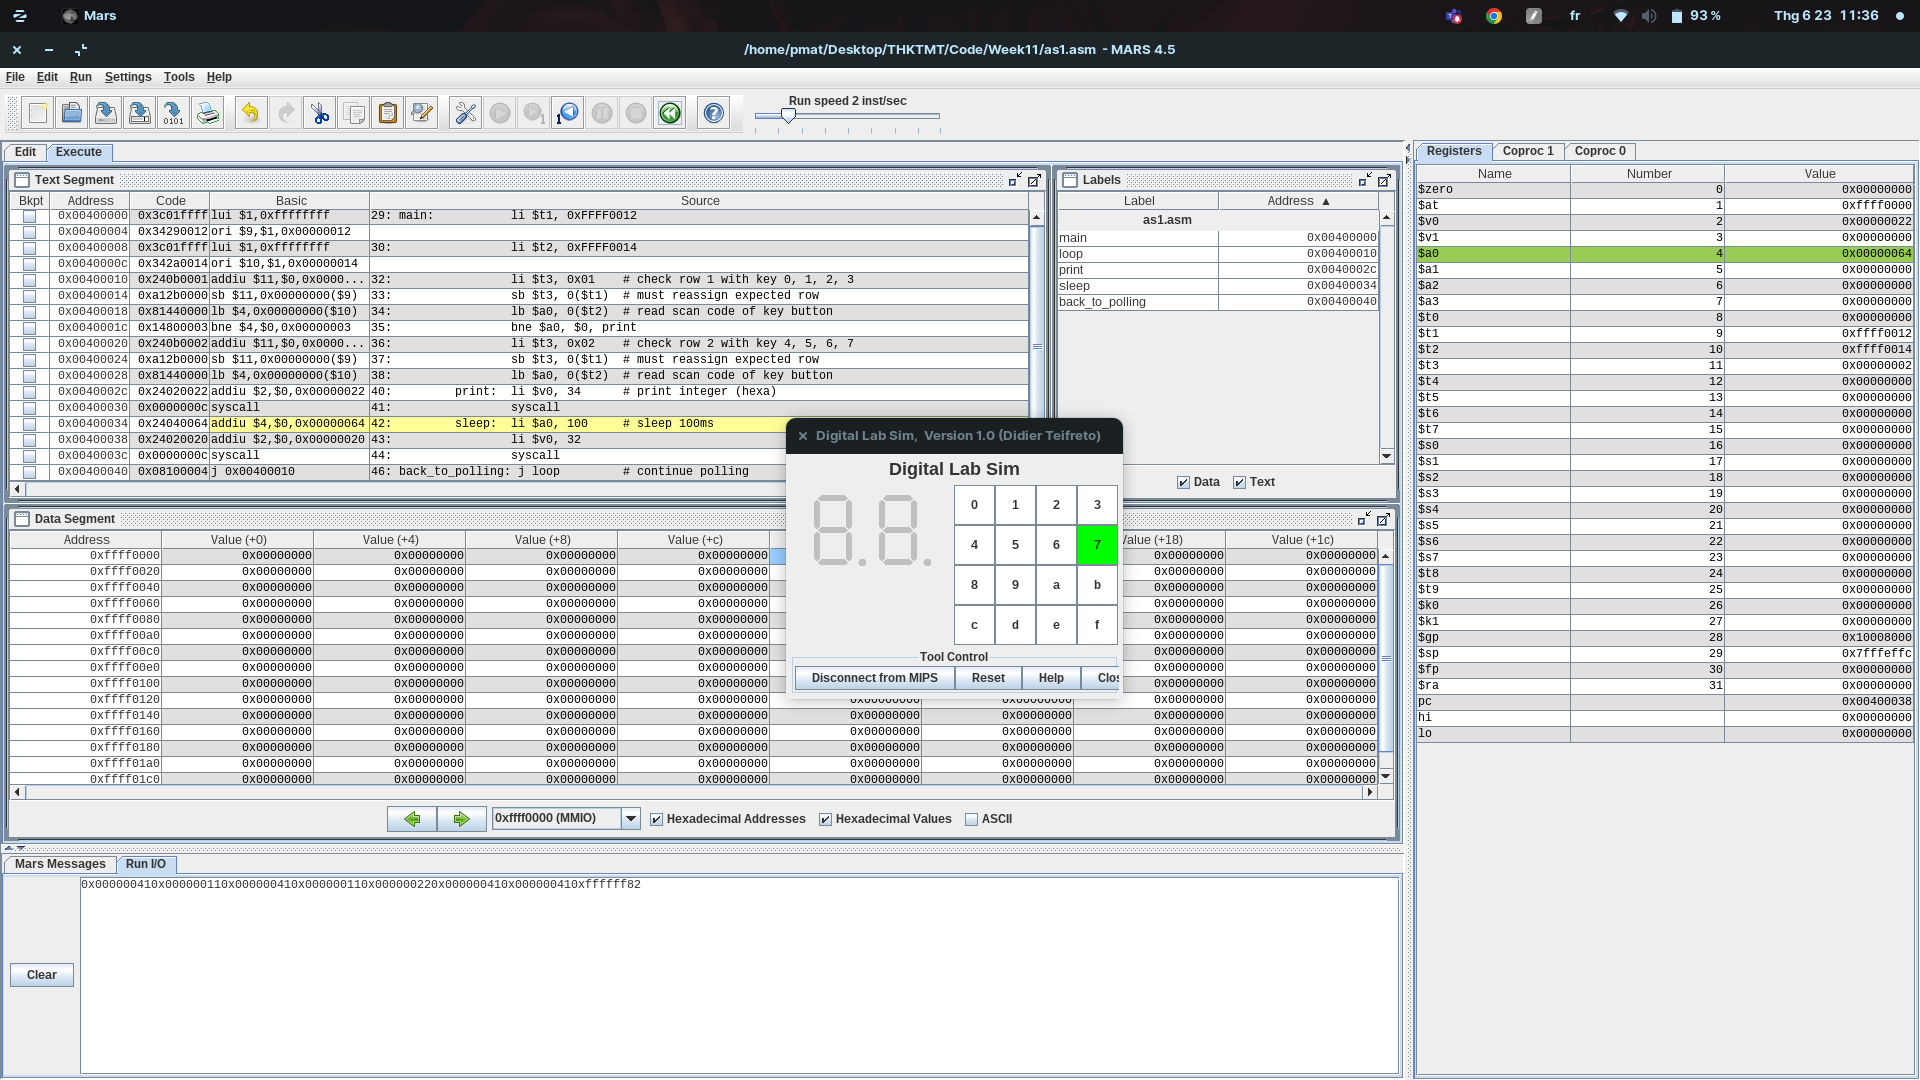
\includegraphics[width=1\textwidth]{ass1/result.png}}}
		\caption{Kết quả của đoạn code}
		\label{fig:ass1}
	\end{figure}
	\noindent
	\textbf{Trong đó:}
	\begin{itemize}
		\item 0x00000041: số 2
		\item 0x00000011: số 0
		\item 0x00000022: số 5
		\item 0xffffff82: số 7
	\end{itemize}
\clearpage
\section{Assignment 2}
\subsection{Phân tích đề bài}
Triển khai ngắt bằng cơ chế Interrupt
\subsection{Triển khai MIPS}
\FloatBarrier
\begin{figure}[ht!]
	\centerline{\fbox{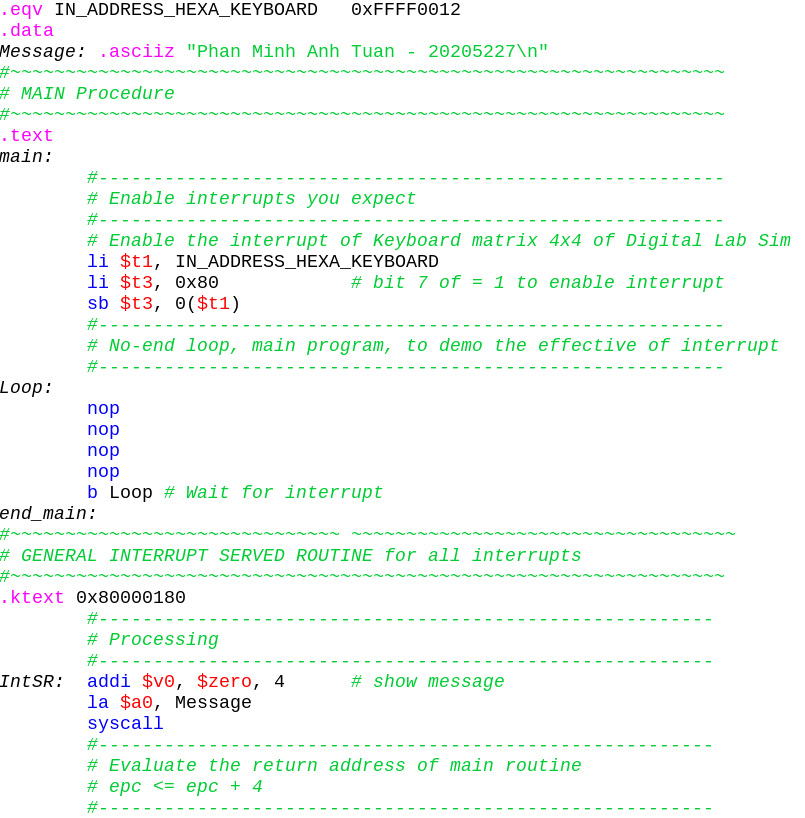
\includegraphics[width=1\textwidth]{ass2/code.png}}}
	\caption*{}
	\label{fig:ass1}
\end{figure}
\clearpage
\FloatBarrier
\begin{figure}[ht!]
	\centerline{\fbox{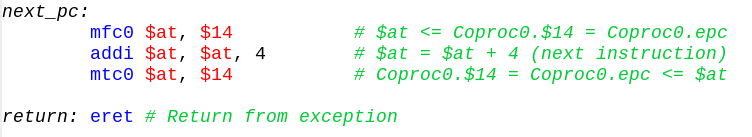
\includegraphics[width=1\textwidth]{ass2/code1.png}}}
	\caption{Code của Assignment 2}
	\label{fig:ass1}
\end{figure}
\noindent
Chương trình thực hiện ngắt khi có một phím bất kì được nhấn bằng cách nạp giá trị vào địa chỉ IN\_ADDRESS\_HEXA\_KEYBOARRD là 0x80, bit số 7 bằng 1 để cho phép ngắt. \\
Khi có một phím được nhấn, chương trình sẽ nhảy địa chỉ cố định 0x80000180 để thực hiện chương trình con phục vụ ngắt. \\
\subsection{Kết quả}
\FloatBarrier
\begin{figure}[ht!]
	\centerline{\fbox{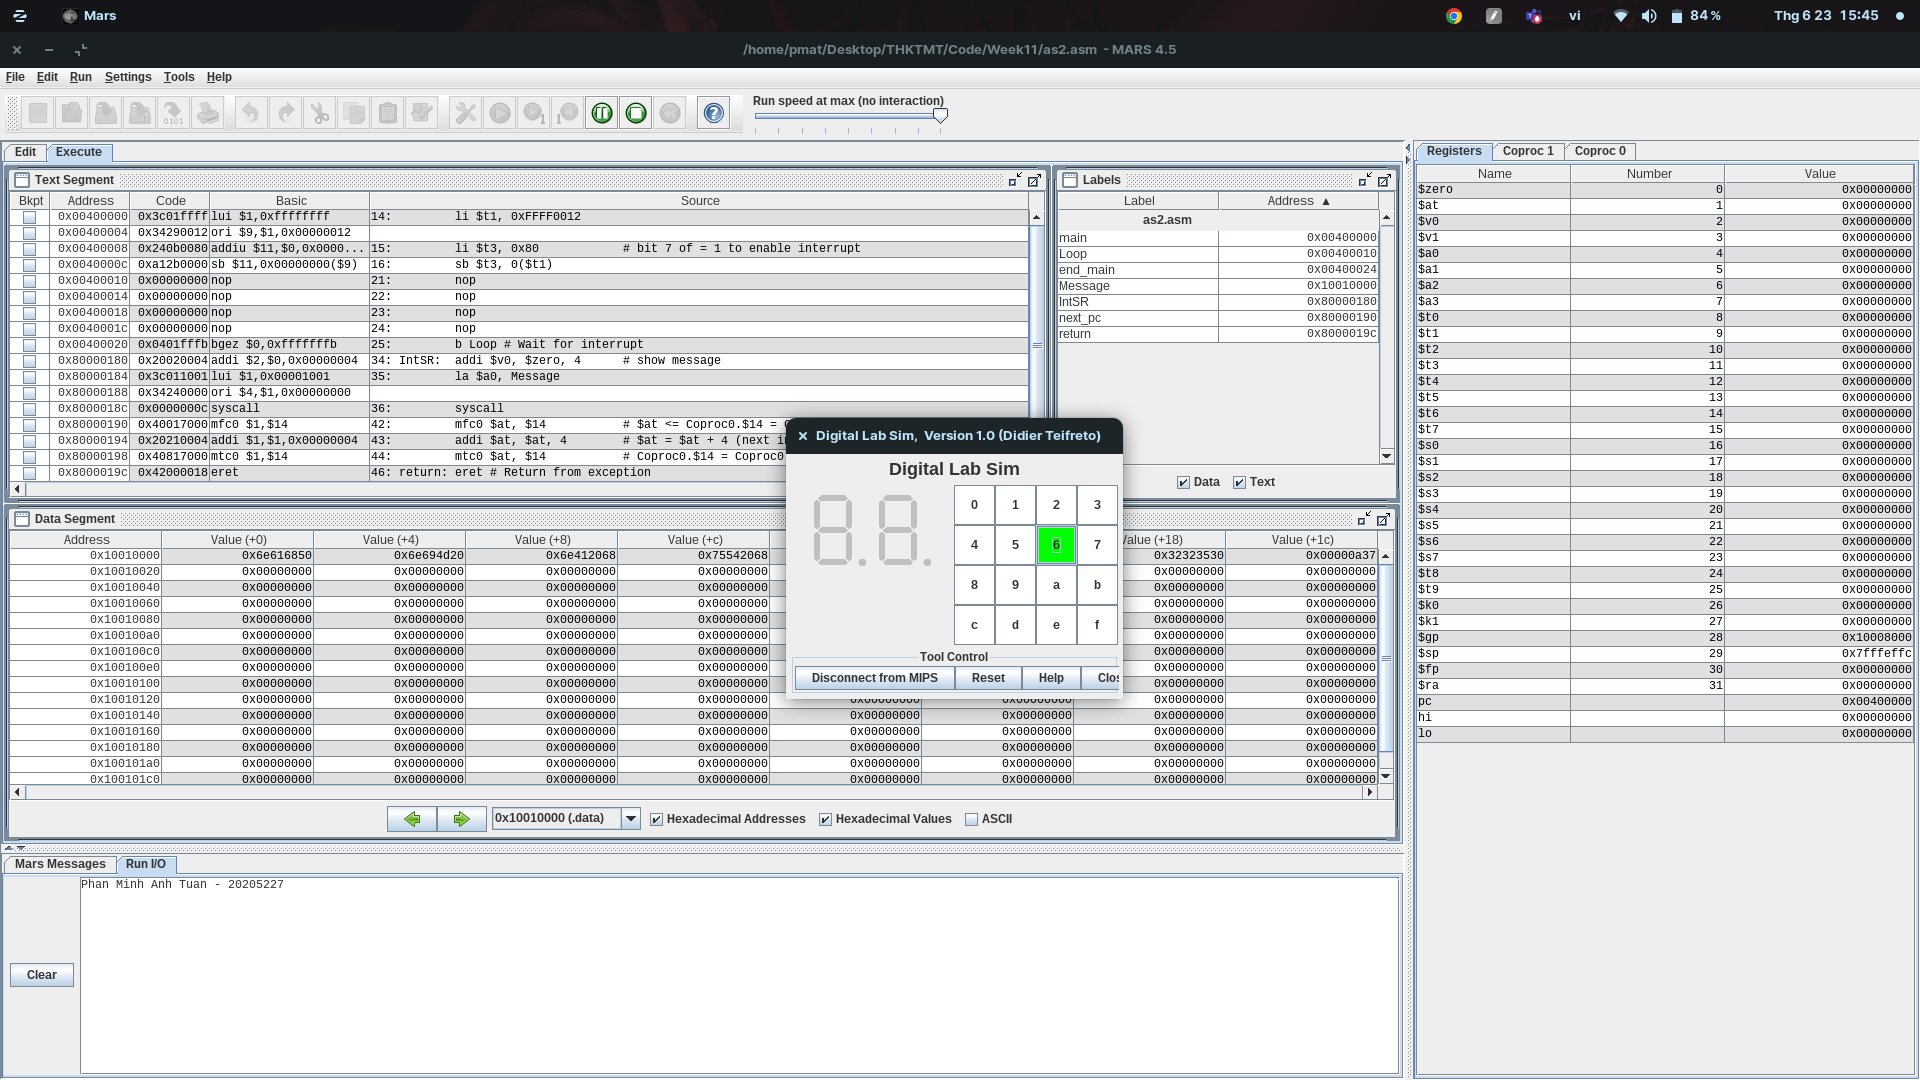
\includegraphics[width=1\textwidth]{ass2/result.png}}}
	\caption{Kết quả của đoạn code}
	\label{fig:ass1}
\end{figure}
\clearpage
\section{Assignment 3}
\subsection{Phân tích đề bài}

\subsection{Triển khai MIPS}
\subsection{Kết quả}
\end{document}